Consider the following system
\begin{center}
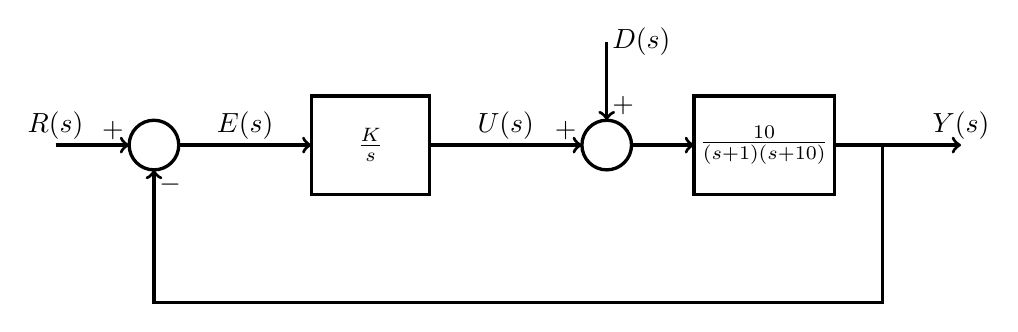
\begin{tikzpicture}[scale=1,inner sep=0pt,outer sep=0pt,very thick,
sysblock/.style={draw,rectangle,inner sep=2pt,minimum width=1.5cm,minimum height=1.25cm,very thick}]

\draw (1.25,0) node[draw,circle] (sum1) {$\rule{0pt}{18pt}$};
\draw (4,0) node[sysblock] (Kp) {$\frac{K}{s}$};
\draw (7,0) node[draw,circle] (sum2) {$\rule{0pt}{18pt}$};
\draw (9,0) node[sysblock] (G) {$\frac{10}{(s+1)(s+10)}$};

\draw[->] (0,0) node[above=2pt] {$R(s)$} -- (sum1.180) node[above left=2pt] {$+$};
\draw[->] (sum1.0) --  node[above=2pt,pos=.5] {$E(s)$} (Kp);
\draw[->] (Kp) -- node[above=2pt,pos=.5] {$U(s)$} (sum2.180) node[above left=2pt] {$+$};
\draw[->] (sum2.0) -- (G);
\draw[->] (G) -- ++(2.5,0) node[above=2pt] {$Y(s)$};
\draw[->] (G) ++(1.5,0) -- ++(0,-2) -| (sum1.-90) node[below right=2pt] {$-$};
\draw[<-] (sum2.90) node[above right=2pt] {$+$} -- ++(0,1) node[right=2pt] {$D(s)$};
\end{tikzpicture}
\end{center}

\begin{enumerate}[(a)]
\item Derive the transfer function from the reference $r(t)$ to the reference error $e(t)$.
\item Find the feasible range for parameter $K$ so that the system is stable and the steady-state error with respect to a unit ramp input $r(t)=tu(t)$ is less than or equal to 0.1.
\item Choose a feasible $K$  and determine the steady state error to a unit step input $r(t)=u(t)$ for that $K$.
\end{enumerate}
